\documentclass[11pt,letterpaper]{article}
\usepackage[T1]{fontenc}
\usepackage[utf8]{inputenc}
\usepackage{lmodern}
\usepackage[margin=1in,headheight=15pt]{geometry}
\usepackage{microtype}
\usepackage{amsmath,amssymb,amsthm,mathtools}
\usepackage{graphicx,booktabs,array,longtable}
\usepackage[dvipsnames]{xcolor}
\usepackage{enumitem}
\usepackage{fancyhdr}
\usepackage{hyperref}
\hypersetup{colorlinks=true,linkcolor=MidnightBlue,citecolor=MidnightBlue,urlcolor=MidnightBlue,
 pdftitle={Exact gaps, parity-dependent zero transitions, and finite-counter recovery},
 pdfauthor={Research prepared for Vladimir Reshetnikov with ChatGPT},
 pdfsubject={Three mathematical extensions of the ProveIt research collection}}
\urlstyle{same}
\setlength{\emergencystretch}{2em}
\setlength{\parskip}{0.25em}
\setlist{topsep=4pt,itemsep=2pt}
\pagestyle{fancy}
\fancyhf{}
\fancyhead[L]{\small Three extensions of the ProveIt methods}
\fancyhead[R]{\small 27 November 2026}
\fancyfoot[C]{\thepage}
\newtheorem{theorem}{Theorem}[section]
\newtheorem{lemma}[theorem]{Lemma}
\newtheorem{proposition}[theorem]{Proposition}
\newtheorem{corollary}[theorem]{Corollary}
\theoremstyle{remark}
\newtheorem{remark}[theorem]{Remark}
\numberwithin{equation}{section}
\begin{document}
\begin{titlepage}
\centering
\vspace*{1.2cm}
{\large RESEARCH REPORT\par}
\vspace{1cm}
{\LARGE\bfseries Exact gaps, parity-dependent zero transitions,\par}
\vspace{0.2cm}
{\LARGE\bfseries and finite-counter recovery\par}
\vspace{0.8cm}
{\large Three extensions of the ProveIt methods\par}
\vspace{0.8cm}
{\normalsize Prepared for Vladimir Reshetnikov with ChatGPT\par}
{\normalsize 27 November 2026\par}
\vspace{1cm}
\begin{minipage}{0.91\textwidth}
\begin{abstract}
We develop three results from the positive-filter, critical-zero, and
spectral-recovery methods in the ProveIt research collection.
First, an exact integer interval certificate determines the largest
zero-free interval for every spectrum
$\pm\{N,(m+1)N,(2m+1)N,(3m+1)N\}$, $m\ge2$.
The nonresonant odd family has a unique eight-atom dual measure and a
supremum not attained on an open interval. This settles an infinite
four-frequency subfamily of Kozma--Oravecz's wide-progression question.
Second, for complete-graph symmetric edge polytopes with a matching
deleted, we resolve the local multiple-root thresholds left open in the
incoming Ehrhart report. Even and odd dimensions have different relative
parameter windows, $(\log d)^{-2}$ and $(\log d)^{-2/3}$, with explicit
quadratic and cubic normal forms and exact local collision parameters.
Third, microscopic histograms of distinct primitive Dirichlet zero
ordinates satisfy a uniform matrix lower bound. It yields optimal
continuous-mixture estimation from exactly $d$ disjoint Poisson counters,
or $d-1$ when the total intensity is known, and a sharp obstruction for
growing bin widths. The three main mathematical results are unconditional.
Dirichlet GRH enters only the identification with the repository's
Li-coefficient semigroups.
\end{abstract}
\end{minipage}
\vfill
\begin{minipage}{0.91\textwidth}
\small
\textbf{Verification status.} Complete analytic arguments, an exact
continuum certificate, independent polynomial certification of the first
four-frequency case, and reproducible symbolic and rational checks are
included. These are research proofs, not new Lean formalizations.
The upstream RH/Dirichlet-GRH development was inspected at source level
but was not rebuilt in this work. Publication priority is subject to
further specialist review.
\end{minipage}
\end{titlepage}
\tableofcontents
\clearpage
\section{Source analysis and the scope of the new results}
\label{sec:overview}

\subsection{What was inspected}
The starting point is the ProveIt directory~\cite{ProveIt}, pinned to
the following commit:
\begin{center}
\texttt{42efb893353a150857f5c8e2f9e7732d0d46f15f}.
\end{center}
Pinning matters because the incoming directory contains results beyond
the merged article. We retrieved and verified the Git blob hashes of
44 article text files, inventoried all 26 current incoming archives,
and extracted their text and code for comparison. The relevant arguments
were read selectively and audited in detail. This is not a claim of
independent verification of the whole 982-page collection.

The article README describes a merger of 209 reports and explicitly
distinguishes merging from mathematical review. Its result labels separate
unconditional statements, uses of Dirichlet GRH, and reductions to
estimates still open. The vendored upstream statements~\cite{GRHLean}
concern the Riemann zeta function and Dirichlet $L$-functions. In particular,
the exported zero-location statement is
\[
 0<\operatorname{Re}s<1,\quad L(s,\chi)=0
 \quad\Longrightarrow\quad \operatorname{Re}s=\tfrac12.
\]
It does not assert simplicity, disjointness of different zero sets,
or GRH for all automorphic or Artin $L$-functions.
We inspected the exported statements and the main source file; we did
not rebuild the vendored development or independently check its full
kernel dependency closure. The new results below do not depend on
endorsing an unperformed verification of that development.

\subsection{The transferable ideas}
Three mechanisms, rather than a blanket appeal to GRH, guide the proofs.

\begin{enumerate}
\item \textbf{Positive annihilators and contact sets.}
A nonnegative trigonometric polynomial and a positive measure whose
Fourier moments vanish give matching primal and dual obstructions.
The new step is a uniform seven-variable contact solution for four
frequencies, together with global positivity and uniqueness.
\item \textbf{Resolve a multiple limiting zero before classifying roots.}
The Ehrhart analogy has an exact reflection line, but a first-order
limit cannot decide what happens at a multiple zero. Retaining the first
nonvanishing corrections produces different quadratic and cubic
transition laws according to parity.
\item \textbf{Turn spectral distinction into a matrix lower bound.}
The earlier binary separation estimate does not by itself control every
real linear combination of several spectra. A joint short-interval
central limit theorem supplies that uniform control. Finite-dimensional
convex geometry then compresses the information into a minimal number
of ordinary count channels.
\end{enumerate}

\subsection{Precise contributions and boundaries}
\begin{center}
\small
\begin{tabular}{@{}>{\raggedright\arraybackslash}p{0.21\textwidth}>{\raggedright\arraybackslash}p{0.40\textwidth}>{\raggedright\arraybackslash}p{0.31\textwidth}@{}}
\toprule
Topic & New result & Boundary \\
\midrule
Four-frequency gaps &
Exact certified analytic characterization for every integer ratio
$m\ge2$, unique eight-atom dual measure for odd $m$, and nonattainment &
An infinite subfamily of Kozma--Oravecz Question 1; arbitrary wide
progressions remain untreated \\
\addlinespace
Ehrhart collisions &
Explicit local critical windows, exact nearby double-root parameters,
and integer-rounding conclusions &
Fixed local clusters, not the global first departure from the
canonical line \\
\addlinespace
Dirichlet mixtures &
Uniform microscopic frame, optimal minimax rate, exactly $d$
counters, and a growing-width obstruction &
Fixed candidate family, known templates and exact bin membership;
no conductor-uniform algorithm \\
\bottomrule
\end{tabular}
\end{center}

The four-frequency result extends the current three-frequency
reports~\cite{ThreeIncoming}; the new odd cases are not the elementary
even-ratio sign-change cases. Its exact description is a uniquely
specified analytic contact system with a finite proof certificate,
not a claimed elementary closed form.
The Ehrhart result answers the local equality and rounding question
explicitly left open in the incoming multipartite report~\cite{EhrhartIncoming}.
The mixture result credits the existing binary Hellinger estimate
of order $T\log T$~\cite{BinaryIncoming}; the new assertions are the
uniform matrix geometry, continuous mixtures, and minimal-count
compression.

Targeted comparisons with the current article, all extracted incoming
reports, and primary literature did not locate these exact extensions.
That is a scoped novelty finding, not an exhaustive publication-priority
certification. The general wide-progression problem, the all-width
complete-bipartite canonical-line question, and the conjectured bounded
excess in positive-filter support are not resolved here.

\subsection{A concrete four-frequency example}
The first nontrivial example is
\[
S=\{\pm1,\pm4,\pm7,\pm10\},\qquad
0.63147839169477181<M(S)<0.63147839169477182.
\]
Approximately, its critical nonnegative polynomial is
\[
\cos\theta+0.66279609635\cos4\theta
0.55610239771\cos7\theta+0.57788131891\cos10\theta.
\]
There are six interior touching zeros and two endpoint zeros on the
critical interval. The dual measure gives positive mass to all eight.
Consequently no polynomial can be strictly positive on that entire
open interval, although a perturbation is positive on every slightly
shorter interval. Figure~\ref{fig:four} displays this distinction.
All decimal bounds claimed as certified are checked by rational interval
arithmetic; plotted coordinates are only illustrations.

\clearpage
\section{Four frequencies in a wide arithmetic progression}
\label{sec:four}

For positive integers $N,m$, let $M_m^{(4)}(N)$ be the supremum of lengths
of intervals on which a nonzero real trigonometric polynomial with spectrum
contained in
\[
 \{\pm N,\ \pm(m+1)N,\ \pm(2m+1)N,\ \pm(3m+1)N\}
\]
does not vanish. Length is measured in $\mathbb R/\mathbb Z$ units. The result
below extends the integer-ratio three-frequency family in the repository's
incoming \texttt{three\_frequency\_gaps.tex}. It is an infinite family of
four-frequency cases of Kozma--Oravecz Question 1~\cite{KO2003}, not a solution for every
arithmetic progression or every number of frequencies. It is unconditional.

For $0\le e\le1/3$ put
\[
 h_e(s)=\begin{cases}\sin(es)/e,&e>0,\\s,&e=0,\end{cases}
 \qquad L_e=\begin{cases}\pi/(2e),&e>0,\\+\infty,&e=0.\end{cases}
\]
The entire extension at $e=0$ is intended in all derivatives. Define
\begin{equation}\label{eq:fourF}
 F_e(s)=h_e(s)+A(e)\cos((1+e)s)+B(e)\sin((2+e)s)
                  +C(e)\cos((3+e)s).
\end{equation}
The coefficients and the four contact parameters $x<0<u<v<w<L_e$ are
specified by the seven equations
\begin{equation}\label{eq:fourcontacts}
 F_e(u)=F_e(v)=F_e(w)=F_e(x)=0,
 \qquad F'_e(u)=F'_e(v)=F'_e(w)=0,
\end{equation}
together with the conditions in the certificate lemma below.

\begin{theorem}[Four-frequency gap formula]\label{thm:four}
For every positive integer $N$ and integer $m\ge2$,
\[
 N M_m^{(4)}(N)=
 \begin{cases}
  1/2,&m\text{ even},\\[2pt]
  1/2-x(1/m)/(\pi m),&m\text{ odd}.
 \end{cases}
\]
For odd $m$, the supremum is not attained even by an open zero-free interval.
For these odd $m$, on the centered critical closed interval, the cone of nonzero nonnegative
polynomials with the stated spectrum is one-dimensional. There is precisely
one annihilating probability measure on that interval: it has eight atoms,
each of strictly positive mass. Here support length means the length of a shortest closed arc containing
the support. For odd $m$, every annihilating measure of minimum support length is a
translate of this one.

There is a real analytic branch of $(A,B,C,u,v,w,x)$ on a neighborhood of
$[0,1/3]$. Consequently the odd-$m$ gap has a convergent expansion in $1/m$
near zero. Its first terms are
\begin{align*}
 N M_m^{(4)}(N)&=\frac12+\frac{c_1}{m}+\frac{c_2}{m^2}+O(m^{-3}),\\
 c_1&=-\frac{x(0)}\pi=0.45356051377648\ldots,\\
 c_2&=-\frac{x'(0)}\pi=-0.18321967877208\ldots.
\end{align*}
In particular,
\[
 0.63147839169477181<M_3^{(4)}(1)<0.63147839169477182.
\]
\end{theorem}

\begin{lemma}[Continuum certificate]\label{lem:fourcertificate}
For every $e\in[0,1/3]$ there is a solution of
\eqref{eq:fourcontacts}, with $-2<x<0<u<v<w<5$, such that:
\begin{enumerate}
\item $w<L_e$, and $F_e\ge0$ on $[x,L_e]$, with zeros exactly
$x,u,v,w$. Moreover $F'_e(x)>0$ and
$F''_e(u),F''_e(v),F''_e(w)>0$.
\item Let the columns of the $3\times4$ matrix $V$ be
\[
 (\cos((1+e)s),\ \sin((2+e)s),\ \cos((3+e)s))^\top,
 \qquad s=x,u,v,w.
\]
All four signed maximal minors $(-1)^j\det V_{\widehat j}$,
$j=0,1,2,3$, are negative.
\item The $4\times4$ matrix with columns
\[
 (\cos(es),\ \sin((1+e)s),\ \cos((2+e)s),\ \sin((3+e)s))^\top,
 \qquad s=x,u,v,w,
\]
has positive determinant.
\end{enumerate}
The Jacobian of the seven equations with respect to
$(A,B,C,u,v,w,x)$ is nonsingular at every solution provided by the certificate.
\end{lemma}

\begin{proof}[How the finite certificate proves the lemma]
In \texttt{checks/spectral}, run:
\begin{verbatim}
python3 -S four_frequency_certificate.py replay
\end{verbatim}
The accompanying
JSON data partition $[0,1/3]$ into 1127 rational cells. Each cell includes a
rational center $z_0$, a positive rational radius $r$, and a rational
$7\times7$ preconditioner $R$. These are proposals, not trusted conclusions.
Let $g(e,z)$ be the vector in \eqref{eq:fourcontacts}, in the script's order,
and set $Z=z_0+[-r,r]^7$. The checker bounds every component of
$R g(e,z_0)$ and every entry of $I-RD_zg(e,z)$ on $E\times Z$ and verifies
\[
 q_i:=\sum_j\sup_{E\times Z}|(I-RD_zg)_{ij}|<1,
 \qquad
 \sup_E |(Rg(e,z_0))_i|+r q_i<r.
\]
For each $e\in E$ the map $z\mapsto z-Rg(e,z)$ is a strict contraction
of $Z$ into its interior. Its unique fixed point is a root of $g$:
$RD_zg$ is invertible by the norm bound, so $R$ is invertible. The same
bound proves nonsingularity of $D_zg$ at the root.

The checker verifies $F'>0$ on a neighborhood of the interval enclosure of
$x$ and $F''>0$ near each of the other three contact enclosures. The known
zero and derivative equations give exact local positivity there. Between
these neighborhoods it uses interval bisection to check $F>0$ through
$\min(9,L_e)$. In a parameter cell with lower endpoint $e_->0$, the
compact check continues to $\min(9,11/(7e_-))$; this covers the needed range
because $\pi<22/7$. The zero lower endpoint is interpreted as an infinite
cutoff. For $9\le s\le L_e$, concavity of sine gives
\[
 h_e(s)\ge 2s/\pi\ge18/\pi>63/11>|A|+|B|+|C|,
\]
where the last inequality is checked on every root box. This proves positivity
on the whole physical interval, including its unbounded limit at $e=0$.
The minor signs and the last determinant are checked directly with interval
arithmetic.

Replay uses only exact integers and rational endpoints. All elementary
operations round outwards to a $10^{-24}$ grid. Sine and cosine are evaluated
at the midpoint divided by sixteen, with Taylor degrees $49$ and $48$,
then four double-angle steps. The remainder is dominated by
$3^{50}/50!<10^{-35}$ on the checked reduced domain, and a grid unit is
added before doubling. The original argument radius is added using the
Lipschitz constant one. The function $\operatorname{sinc} y$ is evaluated
through degree $60$; $4^{62}/63!<10^{-40}$ bounds its remainder on the
checked domain, and its interval radius uses the bound
$|\operatorname{sinc}'y|\le1/2$. Thus the generation routine's floating
point root proposals are not assumptions of the proof.
As a separate check of the first nonresonant member,
\texttt{verify\_m3\_polynomial.py} works in the algebraic coordinate
$y=\cos\theta$ with
\[
 T_1(y)+aT_4(y)+bT_7(y)+cT_{10}(y).
\]
It certifies the seven contact equations, positivity on the whole interval,
positive annihilating weights and the odd-mode determinant using integer
Chebyshev polynomials. This verification uses neither trigonometric
evaluation nor the continuum witness. It therefore supplies an independent
formulation of the $\{1,4,7,10\}$ case.
\end{proof}

\begin{proof}[Uniqueness of the certified branch]
Write $d_j=(-1)^j\det V_{\widehat j}$, with columns indexed by
$(x,u,v,w)$. The four negative signed minors give the positive normalized
null vector
\[
 \lambda_j=\frac{d_j}{d_0+d_1+d_2+d_3}>0,
 \qquad \sum_{j=0}^3\lambda_j=1.
\]
Denote its entries by $\lambda_x,\lambda_u,\lambda_v,\lambda_w$.
Since $F$ vanishes at the four nodes, this vector also annihilates $h_e$.
If two certified solutions had endpoints $x_1<x_2<0$, the first polynomial
would be nonnegative on all four nodes of the second and strictly positive
at $x_2$. Its integral against the second positive rule would be positive,
contrary to annihilation. For equal endpoints the same argument forces the
four contact sets to agree. The nonzero minor obtained by removing $x$
shows that the equations at $u,v,w$ uniquely determine $A,B,C$.

The analytic implicit function theorem applies at every root, by the
nonsingular Jacobian. Solutions from adjacent parameter cells agree at
their shared endpoint by this uniqueness. Local uniqueness from the
implicit function theorem glues the analytic germs. Compactness yields an
open neighborhood of $[0,1/3]$ on which the branch is real analytic.
\end{proof}

\begin{proof}[Proof of Theorem~\ref{thm:four}]
Dilation reduces to $N=1$. When $m$ is even all four frequencies are odd,
so translating by $1/2$ changes the sign of every allowed polynomial.
No zero-free interval can have length greater than $1/2$, and the lowest
cosine has a zero-free open interval of exactly that length.

For odd $m$, set $e=1/m$ and $\theta=2\pi t$. On the positive half of
the centered critical interval let
\[
 s=m(\pi/2-\theta),\qquad
 \theta_* =\pi/2-x(e)/m.
\]
The four terms in \eqref{eq:fourF} are, up to nonzero constant factors,
the allowed cosine modes:
\[
 h_e(s)=m\cos\theta,
 \quad \cos((1+e)s)=(-1)^{(m+1)/2}\cos((m+1)\theta),
\]
\[
 \sin((2+e)s)=-\cos((2m+1)\theta),
 \quad \cos((3+e)s)=(-1)^{(3m+1)/2}\cos((3m+1)\theta).
\]
The certificate therefore gives an even allowed polynomial nonnegative on
$[-\theta_*,\theta_*]$, with precisely the eight zeros
\[
 \pm\theta_s,\qquad \theta_s=\pi/2-s/m,
 \qquad s=x,u,v,w.
\]
Place mass $\lambda_s/2$ at each of these two points. Cosine moments vanish
by the signed-minor construction and sine moments vanish by reflection.
Six atoms lie strictly inside the critical interval. Any allowed polynomial
strictly positive on its open interior has nonnegative endpoint values;
integrating against this measure is therefore strictly positive, a
contradiction. A zero-free polynomial has constant sign, so the same
argument applies after changing its sign. This excludes the critical open
gap as well as every larger gap.

For $x<a<0$, the function $F_e+\delta h_e$ is strictly positive on
$[a,L_e]$ for sufficiently small $\delta>0$. On $[a,0]$ the original
function has a strictly positive minimum, while on $(0,L_e]$ the added
term is positive; $F_e(0)>0$ as well. This is still an allowed cosine
polynomial. Its zero-free interval length tends to $\theta_*/\pi$, proving
the formula and the nonattainment assertion.

Any annihilating probability measure on the critical interval must be
supported on those eight zeros by integration of $F_e$. The paired masses
are uniquely determined by the rank-three projected matrix and mass one.
The differences within the four pairs obey the four sine equations. Up to
row signs and nonzero constants their coefficient matrix is the positive-
determinant matrix in the lemma. Thus all differences vanish and the
measure is unique. Conversely any nonnegative allowed polynomial on this
interval vanishes at every contact. Its odd part is zero by the same
invertible sine matrix, and its cosine coefficients are unique up to scale
by the rank-three condition. This proves the cone assertion. Centering
shows uniqueness up to translation for minimum support measures; smaller
support is excluded by strict positivity on every shorter arc.

Finally expand the analytic function $x(e)$ at zero. The constant values
are specified exactly by \eqref{eq:fourcontacts}; the derivative is
\[
 z'(0)=-\bigl(D_zg(0,z(0))\bigr)^{-1}\partial_e g(0,z(0)),
 \qquad z=(A,B,C,u,v,w,x).
\]
This gives the stated expansion. The decimal figures are numerical
evaluations of the exact branch definition, and are separately enclosed
by the accompanying endpoint calculations.
\end{proof}

\begin{figure}[htbp]
\centering
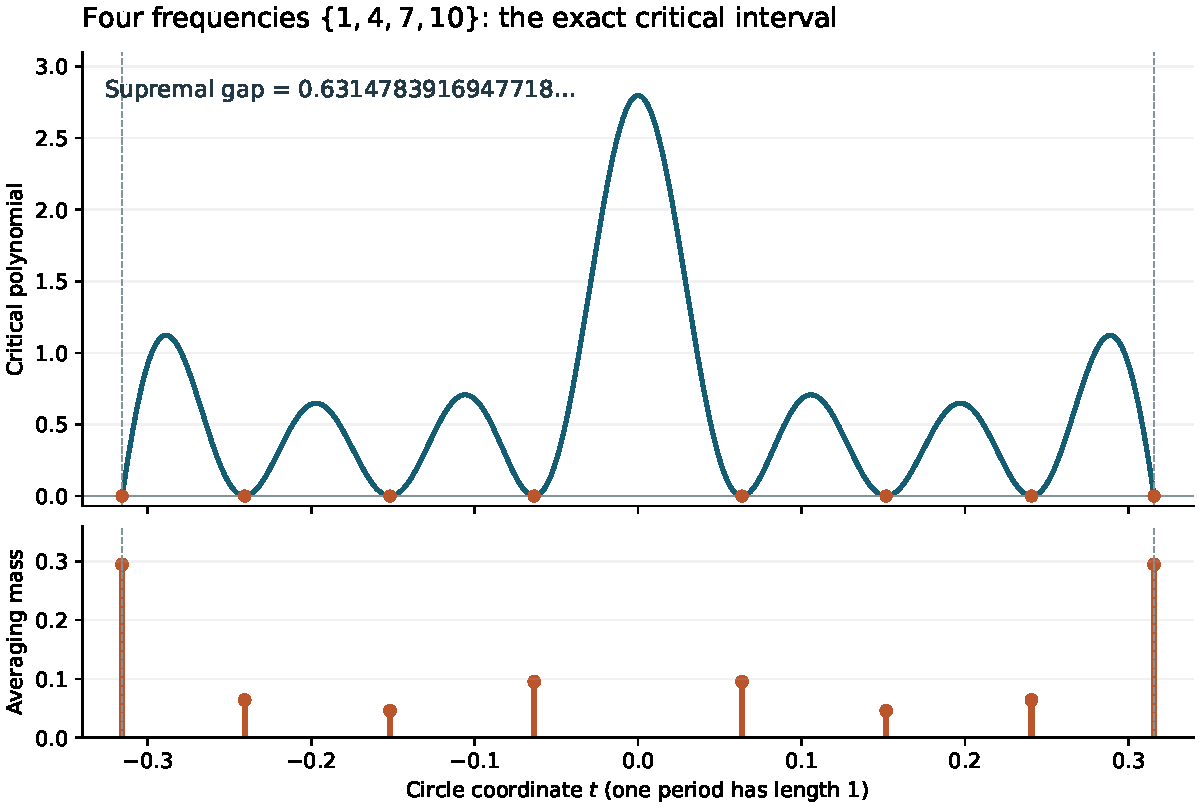
\includegraphics[width=0.97\textwidth]{figures/four_frequency_m3.pdf}
\caption{The certified four-frequency case $\{1,4,7,10\}$.
The drawing uses approximate coordinates; the theorem and exact
certificates establish the contacts, positivity, and dual masses.
The six interior touching zeros explain nonattainment of the critical
zero-free interval.}
\label{fig:four}
\end{figure}
\clearpage
\section{Parity changes the critical exponent of Ehrhart zeros}
\label{sec:ehrhart-critical}

\subsection{The family and what is being resolved}
For $d\ge2$, let $G_{d,M}$ be the complete graph on $d+1$ vertices with a matching of
$M$ edges deleted. For integer $0\le M\le\lfloor(d+1)/2\rfloor$, let
$E_{d,M}(s)$ be the Ehrhart polynomial of its symmetric edge polytope.
The lattice is the integer zero-sum hyperplane, and the polytope is the
convex hull of $\pm(e_i-e_j)$ over the remaining edges. Write $H_d=E_{d,0}$
and let $C_d$ denote the Ehrhart polynomial of the $d$-dimensional
cross-polytope. The exact identity from the incoming multipartite
report~\cite{EhrhartIncoming} is
\begin{equation}\label{ae:exact}
 E_{d,M}(s)=H_d(s)-M D_d(s),\qquad
 D_d(s)=\frac{C_d(s)-C_{d-2}(s)}2. 
\end{equation}
We use \eqref{ae:exact} to define $E_{d,M}$ also for real $M$. This real
interpolation is necessary for discussing an exact collision parameter;
only the integer values are asserted to be graph Ehrhart polynomials.
The eventual collision parameters below are positive and much smaller
than $(d+1)/2$, so rounding them to integers gives legitimate graphs.

For clarity, the matching-deletion identity has a direct lattice-counting
proof. For an integer zero-sum vector $x$, put $q=\sum_i\max(x_i,0)$.
The complete graph gauge is $q$. For a complete multipartite graph the
gauge is
\[
 \max\left(q,\ \max_A\sum_{i\in A}|x_i|\right),
\]
where $A$ runs over its parts. Indeed, direct transport from positive to
negative coordinates has only the same-part restrictions. Hall's
deficiency is $\delta=\max_A(P_A+N_A-q)_+$: a supply set meeting two
parts reaches every demand, so only a single-part set can be deficient.
At most one part has positive deficiency. Send $q-\delta$ units directly
and send the remaining $\delta$ units within that part through an outside
vertex using two edges each. This gives cost $q+\delta$, and the displayed
lower bounds on cost are immediate. The argument also works with real
flows, so it computes the polytope gauge.

For a deleted matching the nontrivial parts are disjoint pairs. A point
of $kP_{K_{d+1}}$ is lost at a pair $\{1,2\}$ precisely when
$|x_1|+|x_2|>k$. It cannot be lost at two pairs, since
$\sum_i|x_i|=2q\le2k$. The two coordinates of a lost pair have opposite
signs. Fix the remaining vector $z\in\mathbb Z^{d-1}$ with positive and
negative masses $P,N$. For one choice of the two signs, write
$x_1=N+c$, $x_2=-P-c$ with $c\ge1$. The lost dilations satisfy
$P+N+c\le k\le P+N+2c-1$. Hence the generating function of the loss
from one pair is
\[
 2\sum_{z\in\mathbb Z^{d-1}}t^{\|z\|_1}
       \sum_{c\ge1}\frac{t^c-t^{2c}}{1-t}
 =\frac{2t(1+t)^{d-2}}{(1-t)^{d+1}}.
\]
This equals the Ehrhart series of $(C_d-C_{d-2})/2$. Additivity of the
disjoint losses proves \eqref{ae:exact} at every nonnegative integer
$s=k$, and therefore as a polynomial identity.

The preceding report established strict subcritical and supercritical
statements at the scale $M\asymp\sqrt d$, and left the equalities out.
The results here describe the previously unresolved local collision
windows. They are unconditional. They use no claim about RH or GRH.
They concern specified clusters of zeros near the canonical line
$\operatorname{Re}s=-1/2$. In particular, ``critical'' below means the
unique collision in that specified cluster, not a claim that this is the
first off-line zero anywhere in the polynomial.

Set
\begin{align}
 L&=\log d,&c_*&=\sqrt{8/\pi},&\beta&=2-\log 2,\label{ae:constants1}\\
 C&=\gamma+\frac53\log2+\frac23,&
 \kappa&=\frac{\pi^2}{4}-2+\frac23(2-\log2)^2.\label{ae:constants2}
\end{align}
Here $\gamma$ is Euler's constant. Numerically,
$C=2.3991276325\ldots$, $\kappa=1.6059772947\ldots$, and
$\kappa\pi^2=15.8503605761\ldots$.
Throughout, $h=(2j+1)\pi$ with a fixed integer $j\ge0$.
The fixed-$j$ condition is essential to the stated error estimates.

\begin{theorem}[The even-dimensional collision]\label{ae:thm-even}
Let $d$ tend to infinity through even integers, and suppose
\[
 M=c_*\sqrt d\left(1+\frac{\alpha_d}{L^2}\right),
 \qquad \alpha_d\longrightarrow\alpha\ne\kappa h^2.
\]
There are precisely two zeros in the corresponding local cluster, counted
with multiplicity, and they satisfy
\begin{equation}\label{ae:even-roots}
 s_\pm=-\frac12+\frac{ih}{L}
 +\frac{-ihC\ \pm\sqrt{\frac23(\alpha-\kappa h^2)}}{L^2}
 +o(L^{-2}).
\end{equation}
The square root may be taken in either order. If $\alpha<\kappa h^2$,
both roots are simple and lie exactly on the canonical line. If
$\alpha>\kappa h^2$, both are simple and off that line, forming a reflected
pair. Their complex conjugates form the corresponding negative-height
cluster.

More precisely, for every fixed sufficiently small neighborhood of
$\alpha=\kappa h^2$, there is for all large even $d$ a unique real local
collision parameter $M^{\mathrm{ev}}_{d,h}$ and collision height
$t^{\mathrm{ev}}_{d,h}$ with
\begin{align}
 M^{\mathrm{ev}}_{d,h}
 &=c_*\sqrt d\left(1+\frac{\kappa h^2}{L^2}+O(L^{-3})\right),
 \label{ae:even-critical}\\
 t^{\mathrm{ev}}_{d,h}
 &=\frac hL-\frac{hC}{L^2}+O(L^{-3}).\label{ae:even-height}
\end{align}
At that parameter the local root has multiplicity exactly two. In the
local neighborhood, increasing $M$ through this value changes two simple
on-line roots into a simple off-line reflected pair.
\end{theorem}

The meaning of ``precisely two in the local cluster'' in this and the next
theorem is unambiguous under rescaling: for any bounded parameter set
separated from its stated transition, choose a sufficiently large fixed
$R$. The cluster is the disk
$|L^2(s+1/2-ih/L)|<R$ in Theorem~\ref{ae:thm-even}, and the disk
$|L^{4/3}(s+1/2-ih/L)|<R$ in Theorem~\ref{ae:thm-odd}.
For all sufficiently large $d$ the indicated number of zeros lies in the
disk, all zeros there have the expansions given, and no zeros lie on its
boundary. A larger fixed $R$ gives the same cluster.

\begin{theorem}[The odd-dimensional cubic window]\label{ae:thm-odd}
Let $d$ tend to infinity through odd integers, and suppose
\[
 M=2c_*\sqrt d\left(1+\frac{\alpha_d}{L^{2/3}}\right),
 \qquad \alpha_d\longrightarrow\alpha.
\]
Define
\begin{equation}\label{ae:alpha-star}
 b=(\beta h)^{1/3},\qquad \alpha_*=-\frac32 b^2.
\end{equation}
If $\alpha\ne\alpha_*$, the cluster consists of exactly three simple
zeros, whose locations are
\begin{equation}\label{ae:odd-roots}
 s_k=-\frac12+\frac{ih}{L}+
             \frac{i x_k}{L^{4/3}}+o(L^{-4/3}),\qquad k=1,2,3,
\end{equation}
where $x_1,x_2,x_3$ are the roots of the explicit cubic
\begin{equation}\label{ae:cubic}
 x^3+2\alpha x-2\beta h=0.
\end{equation}
If $\alpha<\alpha_*$, all three exact zeros lie on the canonical line.
If $\alpha>\alpha_*$, exactly one does, and the other two form an off-line
reflected pair.

There is a unique local real collision parameter and height satisfying
\begin{align}
 M^{\mathrm{odd}}_{d,h}
 &=2c_*\sqrt d\left(1-
       \frac{3(\beta h)^{2/3}}{2L^{2/3}}+O(L^{-1})\right),
 \label{ae:odd-critical}\\
 t^{\mathrm{odd}}_{d,h}
 &=\frac hL-\frac{(\beta h)^{1/3}}{L^{4/3}}+O(L^{-5/3}).
 \label{ae:odd-height}
\end{align}
At this parameter two roots coalesce into a root of multiplicity exactly
two; the third remains simple, at scaled coordinate $x=2b+o(1)$.
In the local neighborhood, increasing $M$ through the collision value
changes three on-line roots into one on-line root and an off-line pair.
\end{theorem}

\begin{corollary}[What happens at the two previously omitted equalities]
\label{ae:cor-equality}
For even $d$, either nearest integer to $c_*\sqrt d$ gives two simple
on-line zeros in each of the fixed clusters in
Theorem~\ref{ae:thm-even}. For odd $d$, either nearest integer to
$2c_*\sqrt d$ gives an off-line pair in each of the fixed clusters in
Theorem~\ref{ae:thm-odd}. In the odd case put $r=(2\beta h)^{1/3}$.
The off-line pair has the explicit form
\[
 s_\pm=-\frac12\pm\frac{\sqrt3\,r}{2L^{4/3}}
       +i\left(\frac hL-\frac{r}{2L^{4/3}}\right)
       +o(L^{-4/3}),
\]
and the remaining zero is
$-1/2+i(h/L+r/L^{4/3})+o(L^{-4/3})$.
\end{corollary}

\subsection{Analytic input, including the resonance at the center}
The argument needs asymptotics in the dimension $d$, not a hypothesis on
arithmetic zeros. The elementary formulas
\begin{align}
 C_d(s)&=\sum_{k=0}^d 2^k\binom dk\binom sk,\label{ae:Cexact}\\
 H_d(s)&=\sum_{k=0}^d\binom dk\binom{d+k}k\binom sk\label{ae:Hexact}
\end{align}
lead to the dimension generating functions
\begin{align}
 \sum_{d\ge0}C_d(s)z^d
  &=(1+z)^s(1-z)^{-1-s},\label{ae:Cgen}\\
 \sum_{d\ge0}H_d(s)z^d
  &=(1-z)^{-1-2s}\,{}_2F_1(-s,-s;1;z^2).\label{ae:Hgen}
\end{align}
One can alternatively obtain \eqref{ae:Hexact} from the complete graph
numerator $\sum_k\binom dk^2 t^k$, followed by coefficient extraction in
its Ehrhart series. These are polynomial identities in $s$; checking the
lattice-counting generating functions for nonnegative integers $s$ proves
them for all complex $s$.

Write $s^*=-1-s$ and
\[
 A(s)=\Gamma(1+s)^{-2},\qquad B(s)=2^s\Gamma(s)^{-1},
 \qquad \epsilon=(-1)^d.
\]
Transfer at $z=1,-1$ in \eqref{ae:Cgen}--\eqref{ae:Hgen} gives
\begin{align}
 H_d(s)&=A(s)d^{2s}+\epsilon A(s^*)d^{2s^*}
             +O(d^{2\operatorname{Re}s-1}+d^{-3-2\operatorname{Re}s}),
 \label{ae:Hasy}\\
 D_d(s)&=B(s)d^{s-1}+\epsilon B(s^*)d^{s^*-1}
             +O(d^{\operatorname{Re}s-2}+d^{-3-\operatorname{Re}s}).
 \label{ae:Dasy}
\end{align}
These estimates are uniform on compact parameter sets avoiding the
resonances $1+2s\in\mathbb Z$; only the extension across $s=-1/2$ is
needed below. For completeness, near $z=1$ the hypergeometric connection
formula yields a singular term
\[
 (1-z)^{-1-2s}\frac{\Gamma(1+2s)}{\Gamma(1+s)^2}
                      (1+O(1-z))
\]
plus an analytic term. The corresponding singular term at $-1$ is
$(1+z)^{1+2s}\Gamma(-1-2s)/\Gamma(-s)^2$ times an analytic factor
with value one. Binomial coefficient transfer gives \eqref{ae:Hasy}.
Multiplying \eqref{ae:Cgen} by $(1-z^2)/2$ gives the generating function
for $D_d$, and the same transfer gives \eqref{ae:Dasy}. Local analytic
terms may be subtracted to any fixed order; both singular expansions and
their remainder bounds are uniform on a compact nonresonant parameter
set. This is the standard two-singularity Darboux argument, equivalently
multiple-singularity transfer~\cite[Chapter VI]{FS2009}; the hypergeometric
connection formulas are recorded in~\cite[Section 15.8]{DLMF}.

\begin{lemma}[Uniform holomorphic error at the resonant center]
\label{ae:lemma-uniform}
Fix $0<\eta<1/4$, a bounded set of $\mu\in\mathbb C$, and write
$s=-1/2+z$, $u=Lz$, $M=\mu\sqrt d$. Then throughout $|z|\le\eta$,
\begin{align}
 dE_{d,M}(-1/2+z)={}& A(-1/2+z)e^{2u}
       +\epsilon A(-1/2-z)e^{-2u}\notag\\
 &-\mu\{B(-1/2+z)e^u
       +\epsilon B(-1/2-z)e^{-u}\}
       +O_\eta(d^{-1+2\eta}).\label{ae:uniform}
\end{align}
On any fixed bounded $u$-disk, the same error bound holds after any fixed
number of $u$-derivatives. It also holds after one $\mu$-derivative;
higher such derivatives vanish.
\end{lemma}

\begin{proof}
The circle $|s+1/2|=\eta$ contains no resonance. On it,
\eqref{ae:Hasy}--\eqref{ae:Dasy}, multiplied by $d$, give the stated
absolute error uniformly for bounded $\mu$; the largest exponent is
$-1+2\eta$. The difference between the two sides of \eqref{ae:uniform}
without its error term is holomorphic in the whole disk. In particular,
the apparent resonance occurs only in the connection formula used to
estimate the boundary; it is not a singularity of that difference.
The maximum-modulus principle extends the bound to the disk. For all
large $d$, a fixed slightly larger $u$-disk maps strictly inside it.
Cauchy's derivative estimates then give all fixed-order $u$-derivative
bounds. The dependence on $\mu$ is affine, and its coefficient has the
same separately proved bound.
\end{proof}

\subsection{The two normal forms}
Define holomorphic functions near zero by
\[
 a(z)=\frac{A(-1/2+z)}{A(-1/2)},\qquad
 b(z)=\frac{B(-1/2+z)}{B(-1/2)}.
\]
Here $A(-1/2)=1/\pi$ and $c_*B(-1/2)=-1/\pi$. Write
\begin{align*}
 a(z)&=1+a_1z+a_2z^2+O(z^3),&
 a_1&=2\gamma+4\log2,&a_2&=\frac{a_1^2}{2}-\frac{\pi^2}{2},\\
 b(z)&=1+b_1z+b_2z^2+O(z^3),&
 b_1&=\gamma+3\log2-2,&b_2&=\frac{b_1^2}{2}-\frac{\pi^2}{4}-2.
\end{align*}
The values follow from the gamma recurrence and
$\psi(1/2)=-\gamma-2\log2$, $\psi'(1/2)=\pi^2/2$.
In particular
\begin{equation}\label{ae:algebra}
 a_1-2b_1=2\beta,\qquad
 \frac{2a_1-b_1}{3}=C,\qquad
 \frac{3C^2-2(a_2-b_2)}2=\kappa.
\end{equation}

For even $d$, put $u=ih+V/L$ and
$\mu=c_*(1+\alpha/L^2)$. Since $e^{ih}=-1$, divide
\eqref{ae:uniform} by $A(-1/2)$ and multiply by $L^2$.
Taylor expansion, using $z=u/L$, gives
\begin{equation}\label{ae:even-normal}
 \frac{L^2d}{A(-1/2)}E_{d,M}
 \left(-\frac12+\frac{ih}{L}+\frac V{L^2}\right)
 =3(V+ihC)^2-2(\alpha-\kappa h^2)+O(L^{-1}).
\end{equation}
The error is uniform on every fixed compact set of complex $(V,\alpha)$,
with all derivatives of any fixed order on smaller compact sets. Indeed,
the Taylor remainder after multiplication by $L^2$ is $O(L^{-1})$,
and the error from Lemma~\ref{ae:lemma-uniform} is
$O(L^2d^{-1+2\eta})=o(L^{-N})$ for every fixed $N$.
One direct way to check the coefficients is to expand first in
$v=u-ih$:
\[
 3v^2+(4a_1-2b_1)zv+2(a_2-b_2)z^2-2\alpha/L^2.
\]
Multiplication by $L^2$, followed by \eqref{ae:algebra}, gives
\eqref{ae:even-normal}.

For odd $d$, put $u=ih+i x/L^{1/3}$ and
$\mu=2c_*(1+\alpha/L^{2/3})$. The normalized leading expression is now
\[
 a(z)e^{2v}-a(-z)e^{-2v}
 -2(1+\alpha/L^{2/3})\{b(z)e^v-b(-z)e^{-v}\},\qquad v=u-ih.
\]
The linear terms in $v$ cancel. The remaining leading terms are
\[
 2v^3-4\alpha L^{-2/3}v+2(a_1-2b_1)z.
\]
Consequently
\begin{equation}\label{ae:odd-normal}
 -\frac{Ld}{2iA(-1/2)}E_{d,M}
 \left(-\frac12+\frac{ih}{L}+\frac {ix}{L^{4/3}}\right)
 =x^3+2\alpha x-2\beta h+O(L^{-1/3}).
\end{equation}
Again the error is holomorphic and locally uniform with every fixed
number of derivatives. Its largest term comes from retaining
$z=ih/L+ix/L^{4/3}$ in the last displayed expression. All other neglected
terms are of the indicated or smaller order. The dimension-asymptotic
error is exponentially small compared with these logarithmic scales.

\subsection{Proof of the collision theorems}
\begin{proof}[Proof of Theorem~\ref{ae:thm-even}]
If $\alpha\ne\kappa h^2$, the limiting quadratic in
\eqref{ae:even-normal} has two distinct roots. Rouch\'e's theorem on
small disjoint circles around them, and on a sufficiently large fixed
circle enclosing both, proves the root count, simplicity, and
\eqref{ae:even-roots}. Reflection across the canonical line preserves
the exact zero multiset, by real coefficients and
$E_{d,M}(-1-s)=(-1)^dE_{d,M}(s)$. When the limiting roots are on the
line, choose reflection-invariant disks centered on that line. Each
contains exactly one exact root counted with multiplicity, so the root
is exactly on-line and simple. When the limiting roots have nonzero
real offsets, their exact roots are off-line for all large $d$.

For the exact collision, set $V=ix$ in \eqref{ae:even-normal}. The
result is real for real $x,\alpha$, and tends in every fixed derivative
norm to
\[
 q(x,\alpha)=-3(x+hC)^2+2(\kappa h^2-\alpha).
\]
The equations $q=q_x=0$ have the solution
$(x,\alpha)=(-hC,\kappa h^2)$. The Jacobian of $(q,q_x)$ with
respect to $(x,\alpha)$ there is
$\left(\begin{smallmatrix}0&-2\\-6&0\end{smallmatrix}\right)$,
which is invertible. The quantitative implicit-function theorem,
or its proof by a contraction on a fixed small neighborhood, gives a
unique nearby solution for the exact functions, with errors $O(L^{-1})$.
This proves \eqref{ae:even-critical}--\eqref{ae:even-height}.
The second $x$-derivative and the $\alpha$-derivative stay strictly
negative. The local graph therefore has a strict nondegenerate maximum,
which crosses zero as $M$ increases. It has two real roots on the lower
side, a double real root at the crossing, and no real roots on the upper
side. The two-root complex count and reflection then give the claimed
off-line pair. The nonzero second derivative also proves multiplicity
exactly two.
\end{proof}

\begin{proof}[Proof of Theorem~\ref{ae:thm-odd}]
The discriminant of \eqref{ae:cubic} is
\[
 -32\alpha^3-108\beta^2h^2.
\]
It is positive, respectively negative, precisely for
$\alpha<\alpha_*$, respectively $\alpha>\alpha_*$. Thus the cubic
has three distinct real roots on the first side, and one real root and
a nonreal conjugate pair on the second. Apply Rouch\'e to
\eqref{ae:odd-normal} as in the even case. In the $x$ coordinate,
reflection across the canonical line is complex conjugation, and the
normalized exact function is real for real $x,\alpha$. The simple-root
uniqueness argument therefore proves exact on-line location, not merely
an asymptotically vanishing displacement, for each limiting real root.

At $\alpha=\alpha_*$, the cubic is $(x+b)^2(x-2b)$. At the double
root $x=-b$, the Jacobian of $(q,q_x)$ is
\[
 \begin{pmatrix}0&-2b\\-6b&2\end{pmatrix},\qquad
 \det=-12b^2\ne0.
\]
The implicit-function theorem gives a unique nearby exact collision
with $(x,\alpha)=(-b,\alpha_*)+O(L^{-1/3})$. This yields
\eqref{ae:odd-critical}--\eqref{ae:odd-height}. Both $q_\alpha$ and
$q_{xx}$ are negative at the double root, so the same local-maximum
argument proves the direction of the transition. The third root stays
simple and real near $2b$. The nonzero second derivative at the colliding
pair gives multiplicity exactly two in the exact finite-$d$ polynomial.
\end{proof}

\begin{proof}[Proof of Corollary~\ref{ae:cor-equality}]
Rounding changes $M$ by $O(1)$. Hence the even rescaled parameter changes
by $O(L^2/\sqrt d)=o(1)$ and the odd one by
$O(L^{2/3}/\sqrt d)=o(1)$. Both limits are therefore $\alpha=0$.
Since $\kappa>0$, this is on the even on-line side; since
$\alpha_*<0$, it is on the odd off-line side. At $\alpha=0$ the cubic
has roots $r,r e^{2\pi i/3},r e^{-2\pi i/3}$, giving the stated formulas.
\end{proof}

\subsection{Exact checks and the limits of the result}
The supplementary programs check the exact polynomial identity, reflection,
and both dimension recurrences by independent rational arithmetic for
small dimensions. They check the Taylor coefficient identities symbolically
and compute local collision parameters with high-precision arithmetic
using the stable real recurrences
\[
 (d+1)^2h_{d+1}=2(2d+1)t h_d-d^2h_{d-1},\qquad
 (d+1)c_{d+1}=2t c_d-dc_{d-1},
\]
where $h_d(t)=i^{-d}H_d(-1/2+it)$ and
$c_d(t)=i^{-d}C_d(-1/2+it)$. These computations illustrate the
convergence; the asymptotic theorems are proved above independently of
the computations.

The result determines local multiplicities, displacement scales, and
collision thresholds for every fixed odd multiple $h$ of $\pi$.
It does not establish the complete bipartite all-width canonical-line
conjecture, a global finite-dimensional graph threshold, a statement
uniform in growing $j$, or an exact critical parameter for integer
$M$ when a real collision lies between consecutive integers. It is a
human-readable mathematical proof, not a Lean formalization. Its novelty
claim is relative to the inspected repository and incoming report;
publication priority has not been exhaustively established.

\clearpage
\section{A uniform frame from binned Dirichlet zero counts}

The new point here is uniformity in every real coefficient vector and in every
microscopic partition.  The binary Hellinger estimate of order $T\log T$ is
already present in the incoming report
\texttt{cycle-complements-and-dirichlet-zero-matching/03-hard-distance-matching}.
It is not claimed as new here~\cite{BinaryIncoming}.  The frame theorem below extends that report
to continuously varying mixtures and yields a minimax estimation theorem.

Let $\chi_1,\ldots,\chi_d$ be distinct fixed primitive Dirichlet characters,
including the conductor-one character if desired.  Count positive ordinates
of nontrivial zeros with multiplicity, without requiring the zeros to lie on
a vertical line.  Put $\mathcal L_T=T\log T$.  Let $\mathcal P_T$ be a
partition of $(T,2T]$ into measurable bins, each of diameter at most
$K/\log T$, where $K<\infty$ is fixed.  Empty bins can be removed, leaving
finitely many bins that contain a zero of the family.  Define
\[
 v_B=(N_1(B),\ldots,N_d(B))^{\mathsf T},\qquad
 s_B=\boldsymbol 1^{\mathsf T}v_B,
 \qquad
 G_T=\sum_{B:s_B>0}\frac{v_Bv_B^{\mathsf T}}{s_B}.
\]

\begin{theorem}[Uniform microscopic frame]\label{mix:thm:frame}
There are $c,C,T_0>0$, depending only on the fixed character family and $K$,
such that for $T\ge T_0$, uniformly over all such partitions,
\[
 c\mathcal L_T I_d\preceq G_T\preceq C\mathcal L_T I_d.
\tag{MF1}
\]
This is an unconditional theorem about zero ordinates.  No assertion about
their simplicity, separation, or noncoincidence is needed.
\end{theorem}

\subsection{The classical input}

Write $C_j(u,h)=N_j(u+h)-N_j(u)$ and let $u$ be uniform on $[T,2T]$.
The short-interval joint central limit theorem of Bombieri and Perelli
\cite[Theorem 2]{BP1998} implies that whenever
\[
 M=M(T)\longrightarrow\infty,\qquad
 M\le\frac{\log T}{\log\log T},\qquad h=M/\log T,
\]
the vector
\[
 Z_T=\left(\frac{C_j(u,h)-M/(2\pi)}{\sqrt{\log M}}\right)_{j=1}^d
\tag{MF2}
\]
converges in distribution to a centered nondegenerate Gaussian vector;
indeed its covariance is $\pi^{-2}I_d$.  The Riemann--von Mangoldt formula
absorbs the fixed conductor terms and the replacement of $\log u$ by
$\log T$ into $O(h+T^{-1})$.

For completeness, the hypotheses in that paper have established
unconditional verification for this family.  The Euler parameters have
modulus at most one, the continuations and functional equations are
classical, and character orthogonality plus the prime number theorem in
fixed residue classes gives their prime orthogonality hypothesis B(IV).
Their density hypothesis D is known for Dirichlet $L$-functions, as explicitly
stated on page 273 of the paper.  Thus (MF2) is not being imported from an
unchecked assertion in the research article.  For $d=1$, one may adjoin a
different primitive character and take a marginal.

We will also use the first-moment consequence
\[
 \mathbb E|C_j(u,h)-C_k(u,h)|=O\bigl(\sqrt{\log M}\bigr)
 \qquad(j,k\text{ fixed}).
\tag{MF3}
\]
This does not follow from weak convergence alone.  It follows from the
$L^1$ approximation by normalized Dirichlet polynomials on page 279 of
\cite{BP1998}, together with the bounded second moments in their Lemma 2.
The fixed conductor drift is $O(h)$ and is negligible.

\subsection{Proof of the frame theorem}

First we prove the uniform $\ell^1$ lower bound
\[
 \sum_B|b^{\mathsf T}v_B|\ge c_1\mathcal L_T\|b\|_2
 \qquad(b\in\mathbb R^d).
\tag{MF4}
\]
Suppose it fails.  Then along a sequence $T\to\infty$ there are allowed
partitions and unit vectors $b_T$ such that
\[
 D_T:=\sum_B|b_T^{\mathsf T}v_B|=o(\mathcal L_T).
\]
Pass to a subsequence with $b_T\to b$, $\|b\|_2=1$, and write
$\delta_T=D_T/\mathcal L_T$.  Choose
\[
 M=\min\left\{\frac{\log T}{\log\log T},
        (\delta_T+\mathcal L_T^{-1})^{-1/2}\right\}.
\]
Then $M\to\infty$ and $M\delta_T\to0$.

Choose one representative $x_B$ in each nonempty bin and move every zero
occurrence in that bin to $x_B$.  Each move has length at most
$K/\log T$.  For a real $x$, the indicator that $x$ belongs to $(u,u+h]$
is supported on the interval $[x-h,x)$ of starting points.  Moving $x$
to $x'$ changes this indicator on a set of measure
$2\min(h,|x-x'|)$.  Therefore, on $u\in[T,2T-h]$,
\begin{align*}
 &\int_T^{2T-h}\left|\sum_j b_{T,j}C_j(u,h)
      -\sum_B b_T^{\mathsf T}v_B\,
                    \boldsymbol 1_{(u,u+h]}(x_B)\right|\,du
 \\
 &\hspace{25mm}\le
 \frac{2K}{\log T}\sum_j|b_{T,j}|\bigl(N_j(2T)-N_j(T)\bigr)
 =O(KT).
\end{align*}
The integral of the absolute value of the second sum is at most $hD_T$.
Thus
\[
 \frac1T\int_T^{2T-h}\left|\sum_j b_{T,j}C_j(u,h)\right|du
 \le M\delta_T+O(K).
\tag{MF5}
\]
The discarded terminal interval of starting points has probability
$h/T=o(1)$.  Divide (MF5) by $\sqrt{\log M}$.  It says that
\[
 a_T+b_T^{\mathsf T}Z_T\longrightarrow0
 \quad\hbox{in probability},\qquad
 a_T=\frac{M\sum_jb_{T,j}}{2\pi\sqrt{\log M}}.
\]
But $b_T^{\mathsf T}Z_T$ converges to a nondegenerate normal law.  If $a_T$
has a bounded subsequence, take a further convergent subsequence to get a
nondegenerate translated normal limit, a contradiction.  If $|a_T|\to\infty$
along a subsequence, tightness of $b_T^{\mathsf T}Z_T$ is a contradiction.
This proves (MF4).

The total mass satisfies $\sum_Bs_B=O(\mathcal L_T)$.  Cauchy--Schwarz gives
\[
 \left(\sum_B|b^{\mathsf T}v_B|\right)^2
 \le\left(\sum_Bs_B\right)
      \left(\sum_B\frac{(b^{\mathsf T}v_B)^2}{s_B}\right),
\]
which proves the lower bound in (MF1).  For the upper bound use weighted
Cauchy--Schwarz separately in every bin:
\[
 \frac{(b^{\mathsf T}v_B)^2}{s_B}
 \le\sum_j b_j^2(v_B)_j.
\]
After summing, each diagonal total is $O(\mathcal L_T)$ by zero counting.
This completes the proof.

\section{Optimal recovery of continuous mixtures}

Suppose independently for each bin we observe
\[
 Y_B\sim\operatorname{Poisson}(t\,\theta^{\mathsf T}v_B),
 \qquad \theta\in[0,R]^d,
\tag{MF6}
\]
where $t>0$ is known and the count vectors $v_B$ are known.  The parameter
$\theta$ specifies an intensity superposition, not a random choice of one
component.  It need not have integer or rational entries.

\begin{theorem}[Minimax rate and an explicit estimator]\label{mix:thm:estimator}
With the setup of Theorem~\ref{mix:thm:frame}, define
\[
 \widehat\theta=\frac1tG_T^{-1}
                  \sum_{B:s_B>0}\frac{v_B}{s_B}Y_B.
\tag{MF7}
\]
Then $\mathbb E_\theta\widehat\theta=\theta$ and
\[
 \operatorname{Cov}_\theta(\widehat\theta)
 =\frac1tG_T^{-1}\left[
     \sum_B\frac{\theta^{\mathsf T}v_B}{s_B^2}v_Bv_B^{\mathsf T}
                       \right]G_T^{-1}
 \preceq\frac RtG_T^{-1}.
\tag{MF8}
\]
If $G_T\succeq c\mathcal L_T I_d$, then for every $u>0$,
\[
 \Pr_\theta\{\|\widehat\theta-\theta\|_\infty\ge u\}
 \le2d\exp\left\{-\frac{ct\mathcal L_Tu^2}{2R+2u/3}\right\}.
\tag{MF9}
\]
Projecting (MF7) onto $[0,R]^d$ gives an estimator whose worst-case squared
Euclidean risk is $O(\min\{1,(t\mathcal L_T)^{-1}\})$.  Conversely, for every
fixed $0<r<R$, even the full unbinned experiment restricted to this band satisfies
\[
 \inf_{\widetilde\theta}\sup_{\theta\in[r,R]^d}
 \mathbb E_\theta\|\widetilde\theta-\theta\|_2^2
 \ge c_{r,R}\min\{1,(t\mathcal L_T)^{-1}\}.
\tag{MF10}
\]
All constants are uniform over the allowed bin partitions.  They depend on
the fixed family, $K,d,r,R$; no conductor-uniform assertion is made.
\end{theorem}

\begin{proof}
The expectation in (MF7) is
$G_T^{-1}\sum_Bv_Bv_B^{\mathsf T}\theta/s_B=\theta$.
Independence and the Poisson variance formula give the equality in (MF8),
and $\theta^{\mathsf T}v_B\le Rs_B$ gives its inequality.

For a fixed coordinate $j$, put
$q_B=e_j^{\mathsf T}G_T^{-1}v_B/s_B$.  Since $v_B$ has nonnegative
coordinates, $\|v_B\|_2\le s_B$, so $|q_B|\le1/(c\mathcal L_T)$.
The centered sum $t(\widehat\theta_j-\theta_j)$ has log moment generating
function
$t\sum_B(\theta^{\mathsf T}v_B)(e^{zq_B}-1-zq_B)$.
The bound
$e^x-1-x\le x^2/[2(1-|x|/3)]$ for $|x|<3$, followed by exponential
Markov, gives a two-sided Bernstein bound with variance parameter at most
$tR/(c\mathcal L_T)$ and maximum jump size $1/(c\mathcal L_T)$.
Substitution and a union bound yield (MF9).  Taking the trace in (MF8)
gives the stated risk.  Coordinatewise clipping cannot increase squared
error relative to any parameter in the box, and bounds it by $dR^2$.

For the lower bound, take two interior points differing by
$\delta e_1$, with $\delta$ smaller than a fixed fraction of $R-r$.
For Poisson laws with means $a,b>0$,
\[
 D_{\rm KL}(\operatorname{Pois}(a)\,\|\,\operatorname{Pois}(b))
 =a\log(a/b)-a+b\le(a-b)^2/b.
\]
Thus, including in the unbinned band experiment,
\[
 D_{\rm KL}(P_\theta\|P_\eta)
 \le\frac{t\delta^2}{r}\sum_B\frac{(v_B)_1^2}{s_B}
 \le\frac{t\delta^2}{r}\sum_B(v_B)_1
 \le C t\mathcal L_T\delta^2.
\]
Choose $\delta$ a sufficiently small constant times
$\min\{1,(t\mathcal L_T)^{-1/2}\}$.  Pinsker's inequality makes the total
variation distance at most $1/2$.  The two-point testing bound for squared
loss then gives (MF10).
\end{proof}

\paragraph{Fisher information and Hellinger geometry.}
For $\theta\in[r,R]^d$ the exact Fisher information matrix is
\[
 \mathcal I_T(\theta)
 =t\sum_B\frac{v_Bv_B^{\mathsf T}}{\theta^{\mathsf T}v_B},
 \qquad
 \frac tR G_T\preceq\mathcal I_T(\theta)\preceq\frac trG_T.
\tag{MF11}
\]
For $\theta,\eta\in[r,R]^d$ the exact squared-root intensity discrepancy
satisfies
\[
 \frac{(\theta-\eta)^{\mathsf T}G_T(\theta-\eta)}{4R}
 \le \sum_B(\sqrt{\theta^{\mathsf T}v_B}
                 -\sqrt{\eta^{\mathsf T}v_B})^2
 \le\frac{(\theta-\eta)^{\mathsf T}G_T(\theta-\eta)}{4r}.
\tag{MF12}
\]
Both inequalities follow by rationalizing each square-root difference.
The Poisson affinity is the exponential of $-t/2$ times this sum.
The new content is the uniform nondegenerate matrix bound, rather than
the standard affinity identity.

\section{Exactly \texorpdfstring{$d$}{d} aggregated Poisson counters suffice}

The estimator (MF7) reduces a large histogram to a $d$-dimensional weighted
statistic, but every bin count still enters it.  A stronger compression is
possible: only $d$ disjoint aggregated count channels need to be retained.
The groups below are selected from the known candidate histograms; they do
not depend on the unknown mixture parameter.

\begin{theorem}[Minimal number of count channels]\label{mix:thm:counters}
For every sufficiently large $T$ and every allowed microscopic partition,
one can choose $d$ disjoint collections of bins
$\mathcal A_1,\ldots,\mathcal A_d$ such that observing only
\[
 Z_k=\sum_{B\in\mathcal A_k}Y_B,\qquad 1\le k\le d,
\tag{MF14}
\]
still gives squared-error risk
$O(\min\{1,(t\mathcal L_T)^{-1}\})$ uniformly on $[0,R]^d$.
These are independent Poisson counters.  The groups may unite bins at
widely separated heights, and all unselected bin counts are discarded.

Conversely, fewer than $d$ fixed disjoint aggregated Poisson counters
cannot identify an unrestricted $d$-dimensional interior box of mixture
parameters, even with arbitrarily long observation time.  This necessity
statement concerns ordinary count channels, not arbitrary real-valued
encodings of an entire dataset.
\end{theorem}

\begin{proof}
Write $p_B=v_B/s_B$, so $p_B$ lies in the probability simplex and
$G_T=\sum_Bs_Bp_Bp_B^{\mathsf T}$.  Let
$G_T\succeq c\mathcal L_T I_d$ and
$\sum_Bs_B\le C_0\mathcal L_T$, with constants from the frame theorem.
Partition the simplex into $J<\infty$ measurable cells of diameter at
most $\delta$, where $C_0\delta^2\le c/4$.  Both $J$ and $\delta$ are
fixed independently of $T$ and of the parameter.

For each nonempty cell $k$, aggregate its bins and put
\[
 S_k=\sum_{p_B\in k}s_B,\qquad
 \bar p_k=S_k^{-1}\sum_{p_B\in k}s_Bp_B,
 \qquad G_T^{\rm cell}=\sum_k S_k\bar p_k\bar p_k^{\mathsf T}.
\]
The exact within-cell covariance identity is
\[
 G_T-G_T^{\rm cell}
 =\sum_k\sum_{p_B\in k}s_B
          (p_B-\bar p_k)(p_B-\bar p_k)^{\mathsf T}
 \preceq C_0\delta^2\mathcal L_T I_d.
\tag{MF15}
\]
Thus $G_T^{\rm cell}\succeq(3c/4)\mathcal L_T I_d$.
Remove cells with $S_k<\eta\mathcal L_T$, where $\eta=c/(4J)$.
Since $\|\bar p_k\|_2\le1$, this removes a matrix of norm at most
$J\eta\mathcal L_T$, leaving a matrix $G_T^{\rm heavy}$ satisfying
\[
 G_T^{\rm heavy}\succeq(c/2)\mathcal L_T I_d,
 \qquad \eta\mathcal L_T\le S_k\le C_0\mathcal L_T
 \quad\hbox{for every remaining cell}.
\]

By Cauchy--Binet,
\[
 \det G_T^{\rm heavy}
 =\sum_{I:\,|I|=d}\left(\prod_{k\in I}S_k\right)
                 \det(P_I)^2,
\]
where $P_I$ has the rows $\bar p_k^{\mathsf T}$, $k\in I$.
Consequently some $d$ remaining cells satisfy
\[
 |\det P_I|\ge
 \kappa:=\left[\binom Jd^{-1}
                   \left(\frac{c}{2C_0}\right)^d\right]^{1/2}>0.
\tag{MF16}
\]
There are at least $d$ remaining cells because their matrix is positive
definite.  Every row has norm at most one, so
$\|P_I^{-1}\|_2\le d^{(d-1)/2}/\kappa$.

Retain precisely these $d$ cell counts.  They are independent with
\[
 Z_k\sim\operatorname{Pois}(tS_k\bar p_k^{\mathsf T}\theta).
\]
The estimator
\[
 \widehat\theta^{\rm count}
 =P_I^{-1}\left(\frac{Z_k}{tS_k}\right)_{k\in I}
\tag{MF17}
\]
is unbiased.  Its covariance is bounded above by
\[
 \frac{R}{t\eta\mathcal L_T}
                P_I^{-1}(P_I^{-1})^{\mathsf T}
 \preceq\frac{R d^{d-1}}{t\eta\kappa^2\mathcal L_T}I_d.
\]
Clipping to the box proves the claimed risk.  If
$A=\|P_I^{-1}\|_{\infty\to\infty}$, the usual Poisson Bernstein bound
also yields
\[
 \Pr\{\|\widehat\theta^{\rm count}-\theta\|_\infty\ge u\}
 \le2d\exp\left\{-\frac{t\eta\mathcal L_T(u/A)^2}
                              {2R+2u/(3A)}\right\}.
\]

Finally, $k<d$ disjoint count channels have a mean vector $tA\theta$ for
a fixed $k\times d$ matrix $A$.  Choose $b\ne0$ in its kernel and two
nearby interior points $\theta$ and $\theta+\varepsilon b$.  Their entire
count vectors have the same law at every $t$.  Thus such a channel system
is not identifiable on any open parameter box.
\end{proof}

This compression theorem uses only the frame bounds and nonnegative
intensity vectors.  The finite-dimensional Poisson argument is therefore
applicable to any family satisfying the same bounds.  The arithmetic
work is what proves those bounds despite shared and clustered zeros.

\begin{corollary}[Known total intensity]\label{mix:cor:normalized}
If $\boldsymbol1^{\mathsf T}\theta$ is known, then $d-1$ disjoint
aggregated counters suffice, with the same risk order on any compact
interior portion of that affine parameter simplex.  Fewer than $d-1$
cannot identify its relative interior.
\end{corollary}

\begin{proof}
Let $P$ be the well-conditioned matrix selected above and write
$\boldsymbol1^{\mathsf T}=c^{\mathsf T}P$.  Since every row of $P$ has
sum one, $\sum_jc_j=d$, so some $c_j\ge1$.  Replace that row of $P$ by
$\boldsymbol1^{\mathsf T}$.  The determinant of the resulting matrix has
absolute value $|c_j\det P|\ge\kappa$, and its row norms are at most
$\sqrt d$.  Use the known total in this row and retain only the other
$d-1$ counters.  The previous covariance argument applies with a zero
variance in the known-total coordinate.  Necessity is the kernel
argument restricted to the $(d-1)$-dimensional tangent hyperplane.
\end{proof}

\section{Why bounded microscopic resolution is the sharp regime}

\begin{theorem}[Collapse at growing bin width]\label{mix:thm:collapse}
Suppose $d\ge2$ and $K(T)\to\infty$.  There are partitions into intervals
of diameter at most $K(T)/\log T$ such that
\[
 \sup_{\substack{\|b\|_2=1\\\boldsymbol1^{\mathsf T}b=0}}
       b^{\mathsf T}G_Tb=o(\mathcal L_T),
 \qquad
 \boldsymbol1^{\mathsf T}G_T\boldsymbol1
       \asymp\mathcal L_T.
\tag{MF13}
\]
Consequently $G_T$ has one eigenvalue of order $\mathcal L_T$ and all
other eigenvalues $o(\mathcal L_T)$.  The same spectral conclusion holds
for $\mathcal I_T(\theta)/t$ uniformly on any fixed interior parameter box.
\end{theorem}

\begin{proof}
Put $m=\min\{K(T),\log T/\log\log T\}$ and $h=m/\log T$.  Partition the
band into intervals of width $h$, with a common origin selected uniformly
in $[0,h)$.  For every $j$, the expected sum over complete cells of
$|N_j(B)-N_1(B)|$ is
\[
 \frac1h\int_T^{2T-h}|C_j(u,h)-C_1(u,h)|du
 =O\left(\mathcal L_T\frac{\sqrt{\log m}}m\right)
\]
by (MF3).  The two boundary cells contribute $O(\log T)$ by the
unit-interval zero bound.  Choose a single origin for which the sum of
these discrepancies over all $j$ is at most its average.  Then
\[
 E_T:=\sum_B\sum_j|(v_B)_j-(v_B)_1|=o(\mathcal L_T).
\]
For $\boldsymbol1^{\mathsf T}b=0$, $\|b\|_2=1$,
$|b^{\mathsf T}v_B|\le\sum_j|(v_B)_j-(v_B)_1|$ and also
$|b^{\mathsf T}v_B|\le s_B$.  Hence
$\sum_B(b^{\mathsf T}v_B)^2/s_B\le E_T=o(\mathcal L_T)$ uniformly
in $b$.  Meanwhile
$\boldsymbol1^{\mathsf T}G_T\boldsymbol1=\sum_Bs_B\asymp\mathcal L_T$.
The eigenvalue assertion follows from the min--max principle and the
general upper bound.  Equation (MF11) transfers it to Fisher information.
\end{proof}

Thus a bounded number of mean zero spacings preserves all mixture
directions up to constant factors.  A growing number can preserve the
overall intensity while losing information at the leading $T\log T$ scale
about every balanced change of composition. Information of smaller order
can still diverge; no impossibility of consistent estimation follows from
this assertion alone. This is a statement about existence of
unfavorable growing-width partitions, not about every such partition.

\section{Application to the symmetric Li processes}

Choose primitive characters $\psi_1,\ldots,\psi_d$ with distinct
conjugacy orbits.  For $\gamma>0$ put
\[
 a_j(\gamma)=m_{\psi_j}(\gamma)+m_{\bar\psi_j}(\gamma).
\]
The symmetric Li process of the repository has rate $a_j(\gamma)/2$ at
each of the two jumps
$\pm2\arctan(1/(2\gamma))$.  For a real character this counts its
multiplicity twice in $a_j$, as required.  Summing the two signs gives
rate $a_j(\gamma)$; the sign is an independent fair mark and carries no
parameter information.  Group these magnitudes by ordinate bins and
use their $a$-count vectors in (MF6).

The frame theorem applies after the injective linear change from the
distinct primitive character family to its disjoint conjugacy-orbit sums.
For example, a coefficient vector on the orbit family expands to the
same coefficient on each member of a nonreal pair and to twice that
coefficient on a real member.  Its Euclidean norm is uniformly comparable
to the original norm because the family is fixed.  Every folded component
has the same leading zero count $(1/\pi)T\log T$, so the collapse theorem
uses the same balanced subspace.

Consequently the mixture estimator, confidence bound, minimax theorem
and sharp coarsening transition apply to intensity superpositions of the
symmetric Li processes.  Dirichlet GRH is used only to identify these
ordinate-built processes with the semigroups defined through the real
Li coefficients.  The histogram frame and its statistical consequences
for the ordinate-built point processes are unconditional.

The angular derivative is
$d[2\arctan(1/(2\gamma))]/d\gamma=-1/(\gamma^2+1/4)$.
On $(T,2T]$, bounded microscopic ordinate bins correspond to angle bins
of width $O(T^{-2}/\log T)$.  The observation model assumes calibrated
candidate zero histograms and exact bin membership.  It makes no claim
that noisy positions can be converted to those counts at the same cost,
and it does not assert an efficient uniform algorithm for constructing
the histograms or explicit constants uniform in conductor.

% Suggested bibliography entry:
% \bibitem{BP1998} E. Bombieri and A. Perelli, Distinct zeros of L-functions,
% Acta Arith. 83 (1998), 271--281, doi:10.4064/aa-83-3-271-281.

\clearpage
\section{Verification, reproducibility, and remaining work}
\label{sec:verification}

\subsection{What the computations establish}
The archive separates exact proof certificates from checks of finite
identities and from numerical illustrations.
\begin{center}
\small
\begin{tabular}{@{}>{\raggedright\arraybackslash}p{0.33\textwidth}>{\raggedright\arraybackslash}p{0.22\textwidth}>{\raggedright\arraybackslash}p{0.36\textwidth}@{}}
\toprule
Artifact & Extent & Logical role \\
\midrule
Continuum interval replay &
1,127 parameter cells; 121,990 positivity boxes &
Proof of existence, global positivity, dual-weight signs, and
nonsingularity for every real $e\in[0,1/3]$ \\
\addlinespace
Independent $m=3$ polynomial certificate &
3,308 positivity boxes &
Separate algebraic formulation using integer Chebyshev polynomials \\
\addlinespace
Point and derivative enclosures &
$e=0$ and eight odd ratios &
Certified displayed gap intervals and first two asymptotic coefficients \\
\addlinespace
Ehrhart exact checks &
172 symbolic or integer checks &
Finite identities, direct lattice counts, normal-form coefficients,
and discriminant; not a replacement for the asymptotic proof \\
\addlinespace
Mixture rational checks &
400 frames and 60 compression cases &
Exact finite-matrix algebra; not verification of the analytic
zero-count theorem \\
\addlinespace
Ehrhart numerical collisions &
Dimensions through 100,001; four 80-digit cross-checks &
Illustrations only; no interval-certification claim \\
\bottomrule
\end{tabular}
\end{center}

The continuum checker uses Python's integer and rational arithmetic only.
Its largest verified contraction bound is less than $0.714$.
Floating-point solvers supply optional proposals during generation;
every proposal is checked independently by the replay routine.
The supplied witness is therefore sufficient without NumPy or SciPy.
Do not disable Python assertions when running the checks.

The gap proof still has a trusted computational base: the short Python
checker, Python's integer arithmetic, the stated elementary remainder
inequalities, and the human-readable mathematical reduction.
It is not a proof object checked by a Lean kernel.
The remaining two results have analytic proofs; their scripts verify
selected exact identities and finite instances.

\subsection{Reproduction}
From the extracted archive root, run
\begin{verbatim}
./build.sh
./verify.sh
\end{verbatim}
The first command builds the PDF with a normal LaTeX installation.
The second replays the exact certificates and the finite algebra checks.
It requires Python and the packages in \texttt{requirements.txt};
the spectral replay itself uses only the standard library.
The optional commands in the component READMEs regenerate illustrations
or perform higher-precision numerical experiments.

The file \texttt{provenance/source\_manifest.json} records the pinned
repository trees. The companion hash report records the 44 retrieved
article text files. The source audit describes the inspected comparisons
and the exact boundary of the upstream-proof inspection.
The archive checksum manifest permits integrity checks after extraction.

\subsection{Natural next mathematical targets}
The first target is an analytic explanation of the four-contact branch
that removes or substantially shortens the interval certificate.
The next spectral extension is five or more frequencies, or a step
ratio not restricted to an integer. Such an extension must control
global positivity and changes in contact pattern, not merely solve
the contact equations numerically.

For the Ehrhart problem, a global root classification would require
uniform control of clusters whose index grows with dimension, together
with exclusion of other departures. The fixed-index normal forms
proved here do not supply that control.

For spectral recovery, explicit conductor-dependent constants and an
observation model with uncertain jump locations would make the
information bounds operational. The present exact-bin theorem does not
automatically imply robustness to positional noise.

These are specific remaining problems. No proof of a broader named
conjecture is inferred from them.

\clearpage
\begingroup
\small
\raggedright
\begin{thebibliography}{20}
\bibitem{ProveIt}
V. Reshetnikov and contributors, \emph{ProveIt, Analysis/GeneralizedRiemannHypothesis},
snapshot at commit \texttt{42efb893353a150857f5c8e2f9e7732d0d46f15f}.
\href{https://github.com/VladimirReshetnikov/ProveIt/tree/42efb893353a150857f5c8e2f9e7732d0d46f15f/Analysis/GeneralizedRiemannHypothesis/}{Pinned repository directory}.
The article and incoming reports are research sources whose verification
status is discussed in Section~\ref{sec:overview}.
\bibitem{GRHLean}
L. Sernau and contributors, \emph{grh-lean}, upstream snapshot
\texttt{72fead102f663d5c7a407964a13dc0cf9d977207},
vendored in the preceding repository. In particular,
\texttt{grh/src/Statements.lean} and \texttt{grh/src/Main.lean}.
\url{https://github.com/lsernau/grh-lean}.
\bibitem{KO2003}
G. Kozma and F. Oravecz, \emph{On the gaps between zeros of trigonometric
polynomials}, Real Analysis Exchange \textbf{28} (2002/03), 447--454.
\url{https://arxiv.org/abs/math/0601021}.
\bibitem{ThreeIncoming}
\emph{Three-frequency gaps}, incoming ProveIt research report,
\texttt{kozma\_oravecz\_three\_frequency\_2026-11-28.zip},
at the pinned snapshot~\cite{ProveIt}. Also see the earlier
\texttt{positive-fourier-zeros.zip}, \texttt{kozma/gaps.tex}.
These establish the prior three-frequency boundary used in the novelty
comparison.
\bibitem{EhrhartIncoming}
\emph{Multipartite Ehrhart research}, incoming ProveIt report,
\texttt{multipartite-ehrhart.zip}, especially \texttt{zeros.tex},
\texttt{combinatorics.tex}, and the concluding questions,
at the pinned snapshot~\cite{ProveIt}.
\bibitem{HKM2017}
A. Higashitani, M. Kummer and M. Micha{\l}ek,
\emph{Interlacing Ehrhart polynomials of reflexive polytopes},
Selecta Mathematica \textbf{23} (2017), 2977--2998.
\url{https://doi.org/10.1007/s00029-017-0350-6}.
\bibitem{DLMF}
NIST Digital Library of Mathematical Functions, Chapter 15, especially
\S15.8 (hypergeometric connection and quadratic transformation formulas).
\url{https://dlmf.nist.gov/15.8}.
\bibitem{FS2009}
P. Flajolet and R. Sedgewick, \emph{Analytic Combinatorics},
Cambridge University Press, 2009, Chapter VI (singularity analysis,
including multiple singularities).
\url{https://algo.inria.fr/flajolet/Publications/book.pdf}.
\bibitem{BP1998}
E. Bombieri and A. Perelli, \emph{Distinct zeros of $L$-functions},
Acta Arithmetica \textbf{83} (1998), 271--281.
\url{https://doi.org/10.4064/aa-83-3-271-281}.
\bibitem{BinaryIncoming}
\emph{Hard-distance matching of Dirichlet zeros}, incoming ProveIt report,
\texttt{cycle-complements-and-dirichlet-zero-matching.zip},
\texttt{03-hard-distance-matching/matching.tex},
at the pinned snapshot~\cite{ProveIt}. This is the prior binary
$T\log T$ Hellinger estimate; that estimate is not claimed as new here.
\end{thebibliography}
\endgroup
\end{document}
